\documentclass[a4paper]{article}

%% Language and font encodings
\usepackage[english]{babel}
\usepackage[utf8x]{inputenc}
\usepackage[T1]{fontenc}

%% Sets page size and margins
\usepackage[a4paper,top=3cm,bottom=2cm,left=3cm,right=3cm,marginparwidth=1.75cm]{geometry}

%% Useful packages
\usepackage{amsmath}
\usepackage{graphicx}
\usepackage[colorinlistoftodos]{todonotes}
\usepackage[colorlinks=true, allcolors=blue]{hyperref}
\usepackage{amssymb}
\graphicspath{	{figures/}	}
\usepackage[font=small]{caption}
\usepackage[labelformat = empty,position=top]{subcaption}
\usepackage[export]{adjustbox}
\usepackage{float}
\usepackage{titling}

\setlength{\parindent}{3em}
\renewcommand{\baselinestretch}{1.5}

\date{}

\title{Creating a gene catalogue for future characterisation of bacterial-fungal community interactions in the oral cavity}

\author{Victoria Butt}

\begin{document}
\pagenumbering{gobble}

\begin{figure}[t]
\centering
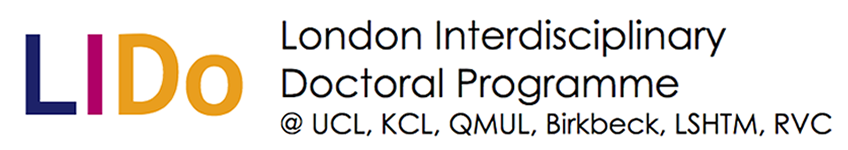
\includegraphics[width=0.7\linewidth,valign=t]{logo.png}

\includegraphics[width=0.2\linewidth,valign=t]{kcl-logo.jpg}
\end{figure}

\maketitle

\newpage
\section{Abstract}
The microbial community residing in the human oral cavity is an essential component of oral health. There have been exhaustive studies investigating the composition of bacterial genes (bacteriome) in the oral cavity, yet fungal genes (mycobiome) are less well-characterised due to their lower abundance and to limitations in DNA extraction methods. To overcome this challenge, a concise catalogue containing both bacterial and fungal genes of the oral cavity will be created by processing and combining three large bacteriome-rich databases with literature searches and open-source datasets of the mycobiome. This catalogue will have several uses. Firstly, genes identified from future shotgun metagenomic sequencing will be mapped against this catalogue to detect low abundance fungal genes as well as bacterial genes. Secondly, this catalogue can also be used directly to generate genome-scale metabolic models (GEMs) for each bacterial or fungal species of interest. GEMs are large-scale metabolic networks that can be simulated \textit{in silico} to infer intra- and inter-species phenotypic interactions. Here, I describe how the gene catalogue is created by trimming, filtering, alignment, assembly and quality control measures, using examples of raw genomic read data from oral samples in the Human Microbiome Project (HMP), a bacteriome-rich database.

\section{Introduction}
The human body has been estimated to be made up of approximately ten times more microbial cells than mammalian cells. The oral cavity is one area of the human body that has a characteristic composition of microbiota that interacts with the human host. In many cases, perturbation in the microbial homeostasis within microbial communities and between microbiota and host, known as dysbiosis, can lead to disease states. Microbes, that are present in a healthy oral cavity but have potential to cause disease, are "pathobionts" that can dominate in this dysbiosis. Pathobiants are microbes that are normally commensal (i.e. obtaining nutrients from the host but not having any harmful nor beneficial effects on the host), but have the potential to become pathogenic from environmental perturbations. \textit{Candida albicans} is an example of a fungal pathobiont which is a dominant pathogen in the common infection, Candidiasis, but is also found as a commensal 50-80\% of healthy human oral cavities \cite{ghannoum_characterization_2010, williams_pathogenesis_2011}.

To begin to fully understand how entire microbial communities in the oral cavity maintain microbial homeostasis in healthy individuals, and how their dysbiosis can lead to infection and disease, all microbial genes existing in the oral cavity should be identified and quantified, and metabolic interactions across different species, should be characterised. In this study, we will focus on identifying and quantifying bacterial (bacteriome) and fungal (mycobiome) genes in the oral cavity, and investigating the metabolic interactions across taxa, including bacteria-fungi interactions.

\subsection{Identifying and quantifying the bacteriome and mycobiome}
Bacterial and fungal genes can be identified and quantified using next-generation sequencing (NGS), a sequencing method that can extract genomic information. In NGS, extracted genomic DNA is sheared into short fragments of approximately 100-1000 base pairs. Both ends of these fragments are ligated with adaptors that are required to initiate the sequencing reaction. These adaptors are extended with primers that attach to a surface to stabilise the fragment, such as a flow cell. During the sequencing reaction, single artificial nucleotides are sequentially bound against a fragment's nucleotide to produce a signal, such as an emission of light or change in pH, specific to the nucleotide type i.e. A, C, G or T. These signals are recorded and processed to create sequences of fragment reads. Algorithms are then used to remove adapter and primer reads or other contamination from these fragment reads. After these filtering procedures, the reads are assembled computationally to create large fragments, known as scaffolds. Other algorithms are then used to identify potential protein-coding genes from these scaffolds.

Extracting the microbial DNA for NGS can be achieved in one of two ways: using a targeted or metagenomic approach. Targeted sequencing is a method of extracting and amplifying specific loci of the genome that contains a great depth of taxonomical and phylogenetic information. The small-subunit ribosomal RNA (rRNA) loci (16S) in bacteria, and the internal transcribed space (ITS) loci (between the small-subunit rRNA and the large-subunit rRNA) in fungi are amplified to sequence bacterial and fungal species. In contrast, metagenomics is defined as the direct analysis of all genomic material contained within an environmental niche \cite{roumpeka_review_2017}. Instead of amplifying specific loci, DNA is extracted and immediately sheared into short fragments for NGS. Many studies have aimed to investigate the diversity of human microbial communities using targeted NGS, especially in the gut \cite{yatsunenko_human_2012, human_microbiome_project_consortium_framework_2012}. Although targeted sequencing is a powerful method of extracting taxonomical information and relative abundance of individual taxa, it has its limitations. Firstly, certain loci have properties where they may be amplified relatively more or less than other loci by PCR, which may create a substantial bias in the relative abundances of the reads, and the subsequent identified taxa. Secondly, targeted sequencing cannot provide detailed information on the true functional diversity in a microbial community. Lastly, this method is limited to taxa for which markers in genetic loci are known and can be amplified. Metagenomic sequencing does not rely on pre-defined loci for amplification, and is free from amplification bias. Crucially, metagenomics can extract a greater diversity of genetic information, and thus resolve functional as well as taxonomical diversity from microbial communities.

Metagenomic analysis has led to the identification of at least 700 bacterial taxa comprising the human oral microbiota \cite{jenkinson_beyond_2011}, but fungal communities still remain less characterised compared to bacterial communities. The composition of the mycobiome has only recently been considered a major component of the human microbiome. It has been estimated 99.1\% of microbial genes were bacterial, with the rest being mostly archae, and only 0.1\% eukaryotic (including fungal) and viral in origin \cite{qin_human_2010,li_integrated_2014}. The mycobiome's contribution to the entire microbiome may be significantly underestimated for several reasons. Firstly, previous estimates have been reliant upon the available annotated microbial reference sequences of which fungi are hugely under-represented. Secondly, a typical fungal cell is 100-fold larger than a typical bacterial cell, meaning fungi account for larger biomass than number of genomes in microbial communities. Thirdly, fungi are eukaryotes that have metabolic features unique from prokaryotes, which may have important roles in microbial homeostasis. Lastly, it is clear that non-bacterial components of the microbiota respond to changes in diet or to dysbiosis, leading to effects in the immune system \cite{devkota_dietary-fat-induced_2012, bull-otterson_metagenomic_2013}.

Several studies have used ITS-targeted sequencing to investigate the oral mycobiome, with some agreement yet significant inconsistencies between them. Dupuy et al.'s discovered \textit{Malassezia} as a prominent commensal, but missed core taxa, \textit{Glomus}, \textit{Teratosphaeria}, \textit{Saccharomycetales} and \textit{Dothioraceae}, which was found by Ghannoum and colleagues previously \cite{ghannoum_characterization_2010, dupuy_redefining_2014}. The potential reasons for these differences between studies are extensive and may be somewhat due to limitations of targeted sequencing methods. To date, there have been no published metagenomic studies of the mycobiome. In the future, we will use metagenomics to quantify the mycobiome as well as the bacteriome.

To be able to quantify the bacteriome and mycobiome using shotgun metagenomic analysis, comprehensive reference catalogues need to be created that contain all possible bacterial and fungal genes that have been found to exist in the oral cavity. Lower abundance genes from metagenomic reads can be detected with higher sensitivity when mapped against a comprehensive reference catalogue, especially for fungal genes. The current catalogue is generated using fragments reads from a total of 682 samples, 382 from the Human Microbiome Project (HMP) \cite{human_microbiome_project_consortium_framework_2012}, 265 from the a rheumatoid arthritis study \cite{zhang_oral_2015} and 35 samples from King's College London [unpublished]. At this stage, a catalogue containing the mycobiome cannot be generated from these databases due to the type of samples, sample collection and library preparation. Instead, this catalogue contains mostly bacterial genes, but fungal genes will be added from external datasets and literature searches at a later date.

\subsection{Inter-species metabolic interactions}

Once the catalogue is complete, it will be used to identify metabolic interactions between species in the oral cavity using computational modelling. Models of metabolic networks need to be built for each of the 50 most abundant species before they can be simulated as follows. The genes within the catalogue will be annotated with their known associated biochemical reactions and metabolites of those reactions. These metabolites will be assembled to create a network of reactions called a genome-scale metabolic model (GEM) \cite{agren_raven_2013, baart_genome-scale_2012}. A GEM can be represented visually by a graph of nodes, representing metabolites, and arrows representing the directions of the reactions. The GEM can also be represented mathematically by a stoichiometric matrix, \textit{S}, where each row and column corresponds to a metabolite and reaction, respectively. Matrix values 1 or -1 correspond to a presence of a reactant or substrate, and 0 corresponds to an absence of a metabolite from a reaction \cite{obrien_using_2015}. To simulate these GEMs, the reactions fluxes, or rate of production or consumption of metabolites, need to be found for each reaction. This is achieved by setting mathematical constraints on metabolite production and consumption, such as setting a limit in the rate of carbon consumed in a reaction. This is known as constraint-based modelling (CBM). The purpose of CBM is to reduce the search space of the number of possible flux combinations that could occur, avoid non-physiological fluxes and reproduce similar environments seen \textit{in vivo} \cite{magnusdottir_generation_2017, bordbar_constraint-based_2014}. Next, a mathematical objective function is defined which aims to maximise (or minimise) the production of a particular metabolite or cellular phenotype. The fluxes are found by simulating the GEM with its constraints and objective function using optimisation algorithms, such as linear programming. To find inter-species interactions, the GEMs are paired and simulated together as described to find the pairwise fluxes, and thus the inter-species metabolic interactions.

Here, I describe the pipeline for creating the catalogue, looking specifically at processing the metagenomic reads of nine samples taken from the bacteriome-rich database, the HMP, and showing how quality control measures can identify and remove poor quality samples.

\section{Materials and Methods}

The pipeline for creating the gene catalogue from bacteriome-rich databases is described below. Nine samples, taken from the HMP database, are used here as an example of the entire analysis for all 682 samples from HMP \cite{human_microbiome_project_consortium_framework_2012}, the rheumatoid arthritis study \cite{zhang_oral_2015} and King's College London [unpublished]. The samples, SRR060075, SRR060076, SRR060040, SRR064436, SRR060154, SRR061324, SRR061359, SRR061490 and SRR061492, were downloaded from NCBI: \url{ftp://ftp.ncbi.nlm.nih.gov/sra/sra-instant/reads/ByExp/sra/SRX/SRX023/} and \url{ftp://ftp.ncbi.nlm.nih.gov/sra/sra-instant/reads/ByExp/sra/SRX/SRX024/}
These files contain paired-end reads of sequenced DNA from the oral cavity that were sequenced from an Illumina HiSeq 2000. The following pipeline was run on a high performance cluster computer, ``Rosalind" at King's College London. Refer to Supplementary Code (SC) \url{https://github.com/blue-moon22/lido-thesis-2017} for code and parameters used.

\begin{figure}[H]
\centering
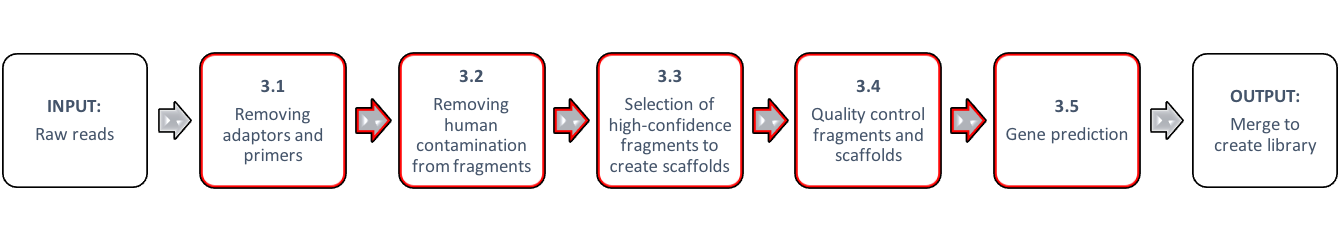
\includegraphics[width=\linewidth,valign=t]{workflow.png}
\caption{\label{fig:workflow} Pipeline for creating the gene catalogue}
\end{figure}

\subsection{Removal of adapters and primers from fragment reads}
The raw reads for each sample were trimmed using AlienTrimmer (Version 0.4.0) \cite{criscuolo_alientrimmer:_2013}. AlienTrimmer was used to detect and remove contaminant sequences, adapters and primers, that are found at both ends of the reads and used as part of the sequencing protocol (SC Step 1).

\subsection{Removal of human contamination from fragment reads}
Human contaminant sequences were removed from the reads, since we are only interested in identifying microbial genes. This was achieved by mapping the reads against a human reference genome using Bowtie2 (Version 2.2.3), and removing those sequences that successfully matched with the human reference genome (SC Step 2). Bowtie2 aligns sequence reads to long reference sequences using memory-efficient algorithms based on the Burrows-Wheeler Transform \cite{langmead_aligning_2010}.

\subsection{Selection of high-confidence fragments to create scaffolds}
To ensure the reads are completely derived from bacterial (and fungal) species and devoid of any other contamination, an additional filtering step was included (SC Step 3). Using Bowtie2, a reference genome was built from assembled scaffolds. These scaffolds were assembled from the trimmed and filtered fragment reads (generated in 3.2) using SPAdes (Version 3.9.0). SPAdes is a genome assembler tool based on resolving de Bruijn graphs, and specialises in single-cell bacterial and fungal read assemblies \cite{bankevich_spades:_2012}. As the reads are metagenomic, the metaSPAdes pipeline was used for this assembly \cite{nurk_metaspades:_2017}. Again, using Bowtie2, the trimmed and filtered reads generated from 3.2 were aligned against the built reference genome. Different scaffolds were generated from fragment reads that aligned, and those reads that did not align were removed. The name, length, and number of mapped reads in each of these scaffolds were extracted using SAMtools (Version 1.3.1), a software tool used to read or write file formats containing scaffold information, and extract scaffold statistics \cite{li_sequence_2009}. Scaffolds with a length of less than 500 and containing less than 11 mapped reads were removed.

\subsection{Quality control fragments and scaffolds}
The quality of sequencing and the amount of contamination of the samples were considered as different quality control measurements. The quality of sequencing was measured by counting the number of fragment reads before and after trimming in 3.1. A large decrease in the number of reads may suggest problems with the sequencing protocol. The amount of contamination of the sample was measured by counting the number of fragment and scaffold reads before and after removal of potential contamination in 3.2 and 3.3. A large decrease in the number of reads may suggest a large amount of contamination. The measurements were calculated by dividing each count by the total pre-processed fragment/scaffold count for each sample, and multiplying by 1,000,000 to give the normalised read count per million (RPM) (SC Step 4). Samples with outlier counts were excluded from the gene catalogue.

\subsection{Gene predictions}
The filtered scaffolds for each sample that passed quality control was merged into one fastq file (SC Step 5). Bacterial genes from this file were identified using Prodigal (Version 2.6.3), a protein-coding gene prediction software, mainly used for bacterial and archaeal genomes \cite{hyatt_prodigal:_2010}. Alternative software will be required to identify eukaryotic genes for future construction of the mycobiome content of the catalogue. Gene lengths of less than 60 and genes containing mycoplasm/spiroplasm code or mold, protozoan and coelenterate mitochondrial code were removed. This left potential bacterial (and archaeal) genes only. To create the final catalogue, the filtered genes were clustered using CD-HIT (Version 4.6.6), a greedy incremental clustering algorithm that is used to cluster sequences to remove redundancies \cite{li_cd-hit:_2006}.

\section{Results}

\subsection{Quality control identifies outliers}

A catalogue of bacterial genes was created from metagenomic reads of oral cavity samples taken from three bacteriome-rich databases. In the future, the catalogue will be used for addition of fungal genes to identify and quantify both the bacteriome and mycobiome in the oral cavity, and to investigate inter-species metabolic interactions across bacteria and fungi. To generate a reliable gene catalogue from metagenomic reads, the samples were quality controlled. Out of the nine samples from the HMP, eight were considered high quality and could be included as part of the final catalogue. The quality of sequencing and the amount of contamination of the samples were considered as different quality control measurements, with the quality of sequencing being the most important one. The quality of sequencing was quantified as the change in fragment reads per million (RPM) before and after trimming away adapter and primer reads from the fragments (first and second columns of Fig. 2a). The amount of contamination of the samples was quantified as the change in fragment and scaffold RPM before and after removal of potential (human) contamination (second and third columns of Fig. 2a, and both columns of Fig. 2b). Sample SRR060154 has the highest RPM of pre-processed raw reads and the greatest decrease after trimming compared to other samples in Fig. 2a. This sample's reads contained a high amount of adapters and primers, meaning there may have been problems with the sequencing protocol. Both Fig. 2a and 2b, show a relatively uniform distribution of fragment and scaffold RPMs before and after removal of contamination. Since the quality of the reads are most dependent on the quality of the sequencing, sample SRR060154 was excluded from the catalogue.

\begin{figure}[H]
\centering
\begin{subfigure}[t]{0.03\textwidth}
\textbf{a)}
\end{subfigure}
\begin{subfigure}[t]{0.95\textwidth}
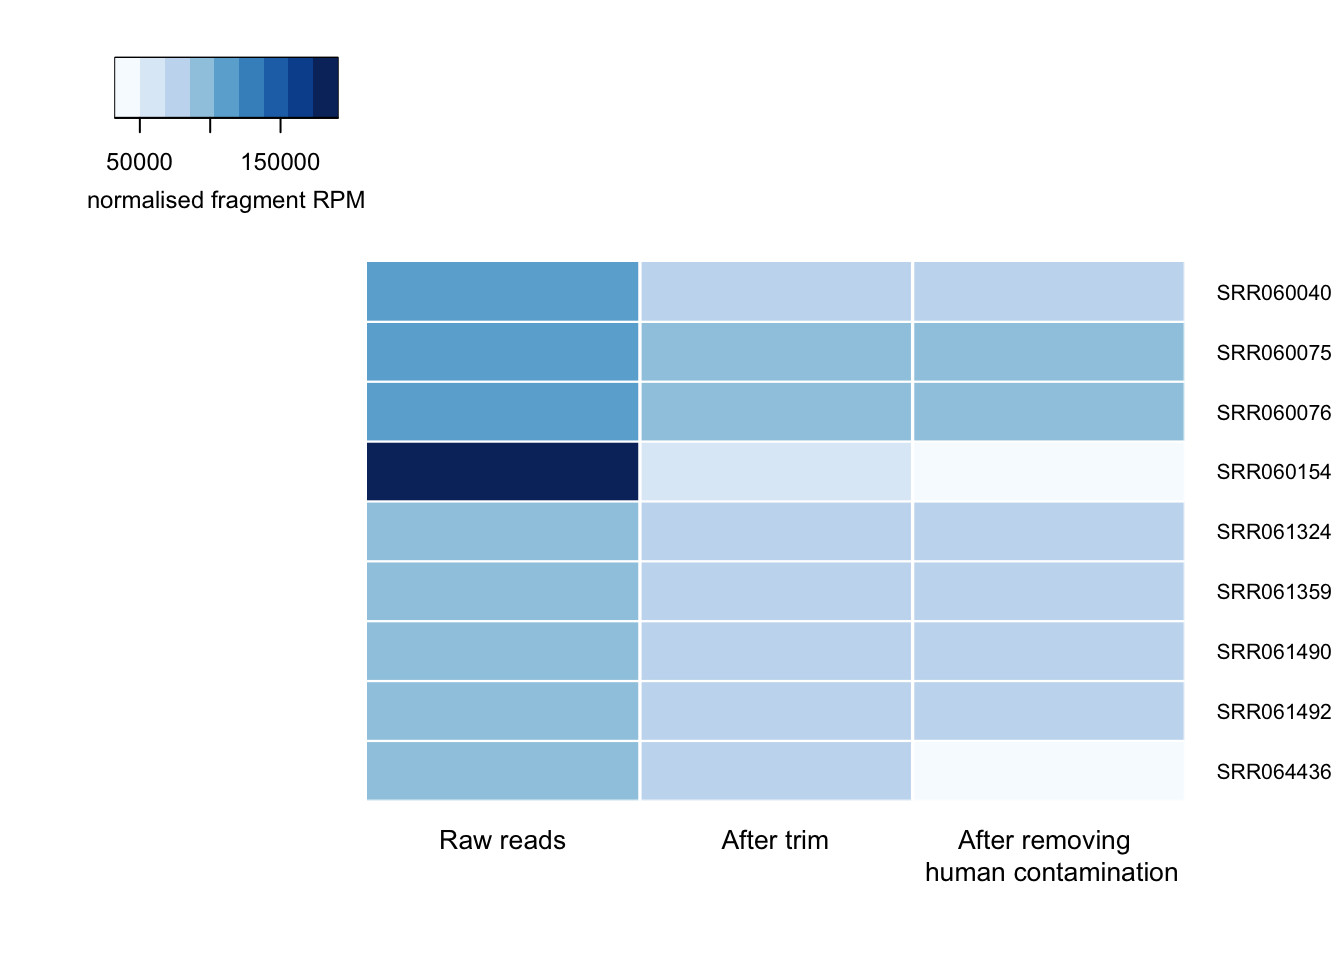
\includegraphics[width=\linewidth,valign=t]{fragment_heatmap-1.png}
\end{subfigure}\hfill
\begin{subfigure}[t]{0.03\textwidth}
\textbf{b)}
\end{subfigure}
\begin{subfigure}[t]{0.95\textwidth}
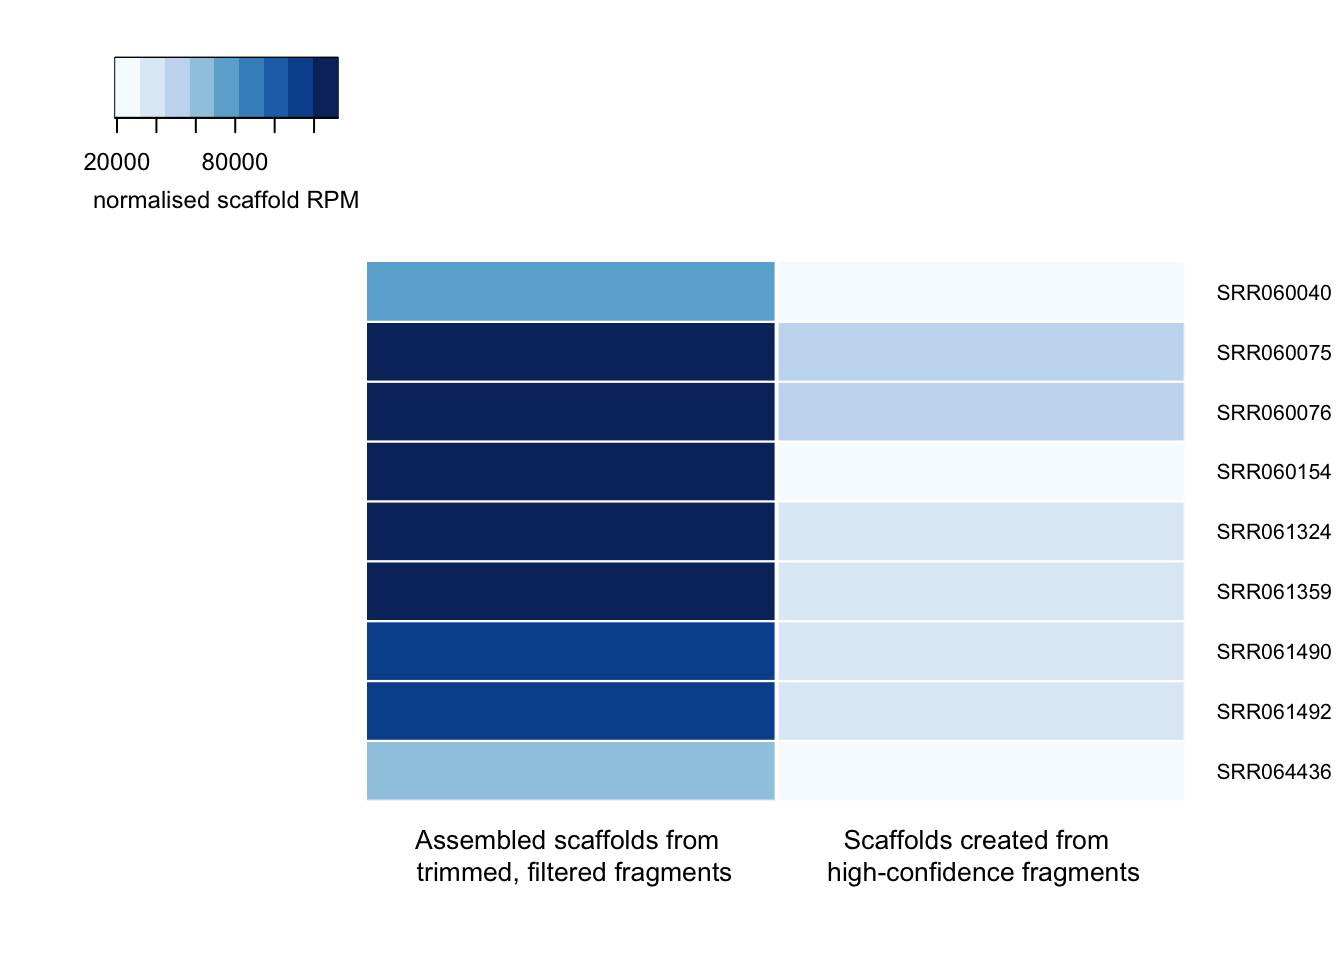
\includegraphics[width=\linewidth,valign=t]{scaffolds_heatmap-1.png}
\end{subfigure}

\caption{\label{fig:quality control} For each of the nine samples, the normalised reads per million (RPM) of a) fragment reads before and after each filtering step: before trimming (pre-processed raw reads), after trimming by AlienTrimmer, and after removal of human contamination; b) scaffolds assembled from trimmed and filtered fragments, and scaffolds created from high-confidence fragments aligned to a reference genome built from the assembled scaffolds}
\end{figure}

\section{Discussion}
In metagenomic studies of the human microbiome, there has been a no coverage to date of the fungal genome for several reasons. Firstly, there are very few comprehensively annotated catalogues of fungal genes in the human microbiome. Secondly, many common DNA extraction protocols are limited in extracting fungal DNA due to the difficulty in breaking melanin in some fungal cell walls. Several studies have successfully extracted fungal DNA using several different protocols, but the species predictions have not been completely consistent \cite{vesty_evaluating_2017}.

We will overcome the first issue by creating a comprehensive catalogue of both bacterial and fungal genes that exist in the oral cavity. At present, the catalogue has been successfully generated from the pipeline to include mostly bacterial genes, and fungal genes will need to be added at a later stage from external, open-source datasets and literature searches. To address the second issue, we will be investigating various DNA extraction protocols that are optimised for extracting fungal DNA from saliva for metagenomic analysis. Thus far, we have attempted to extract fungal DNA using an adapted extraction method described previously \cite{furet_comparative_2009} and the MoBio PowerSoil DNA Isolation Kit, with limited success. We will  trial other extraction protocols, including MolYsis as described previously \cite{mccann_evaluation_2014} and other protocols from studies that have extracted fungal DNA for ITS-targeted sequencing. It is hoped the final optimised protocol will be used to extract bacterial and fungal DNA from human saliva samples, and mapped against the catalogue to give a personalised profile of the bacteriome and mycobiome for an individual.

GEMs can be created from the current bacterial gene-rich catalogue for each bacterial species present, and can be computed to infer large-scale bacterial community interactions in the oral cavity. To aid the precision of the GEMs, transcriptomic data will also be integrated into the catalogue to determine the expression status of a gene, identify potential gene isoforms that confer different metabolic functions and to consider any metabolic feedback loops. Once the fungal genes are added to the catalogue, the GEMs can be iterated to include fungal community interactions as well as bacterial. As well as being able to model metabolic interactions on a large scale, GEMs have the potential to generate a profile of anti-microbial resistance genes (ARGs) in the microbial community, also known as the "resistome" \cite{wright_antibiotic_2007}. ARG profiles would allow identification of genes involved in the resistance of antimicrobial drugs, especially genes where their involvement is not obvious from targeted studies. Novel antibiotics can be developed based on these anti-microbial genes products, which have potential to tackle the current and future world's antibiotic-resistance crisis. At a later stage, optimised DNA extraction methods and metagenomic shotgun sequencing of human saliva samples could generate personalised GEM profiles for an individual. Using personalised GEMs that are modelled to an individual's microbial community could reveal how an individual's microbiota will affect their response to certain antimicrobial drugs.

In the future, a comprehensive gene catalogue of the bacteriome and mycobiome, and its uses in accurate fungal and bacterial species identification and creation of GEMs, has the potential to identify therapeutic targets, such as influential genes that could be targeted by novel antimicrobial drugs, and diagnostic biomarkers to give precise disease status.

\section{Acknowledgements}
I would like to thank my supervisors, Dr David Moyes and Dr Peter Mullany for their support, Dr David Gomez-Cabrero Lopez for sharing the code, Dr Elizabeth Witherden for help with fungal DNA extraction, and Dr Saeed Shoaie for information on GEMs.

\newpage
\bibliographystyle{ieeetr}
\bibliography{rotation_refs}

\end{document}